\chapter[BRT]{Boosted Regression Trees}

\begin{objetivos}
	Ao final desta unidade, o estudante deverá compreender os fundamentos das Boosted Regression Trees; ajustar modelos BRT para dados presença-background; controlar hiperparâmetros para reduzir sobreajuste; selecionar o número ótimo de árvores por validação cruzada; avaliar o modelo com AUC, TSS, sensibilidade e especificidade; interpretar importância relativa das variáveis; gerar curvas de resposta parcial; produzir mapas de adequabilidade ambiental de \textit{Dinizia excelsa}; e comparar BRT com GLM, GAM e Random Forest.
\end{objetivos}

\section{Introdução}

Boosted Regression Trees, ou BRT, combinam árvores de decisão com boosting. Diferentemente do Random Forest, que ajusta muitas árvores independentes e combina suas predições, o boosting ajusta árvores sequencialmente, de modo que cada nova árvore tenta melhorar os erros deixados pelas árvores anteriores. Em SDM, BRTs são amplamente usadas porque capturam respostas não lineares, interações entre variáveis e padrões ambientais complexos \parencite{elith2008working,elith2009,guisan2017habitat}.

\begin{conceito}[title={\faBook\quad BRT em SDM}]
	BRT é um algoritmo flexível que combina árvores de decisão e aprendizado sequencial. Ele pode representar relações ecológicas complexas, mas exige controle rigoroso de hiperparâmetros para evitar sobreajuste.
\end{conceito}

\section{Hiperparâmetros principais}

Os principais hiperparâmetros em BRT são:

\begin{itemize}
	\item \texttt{n.trees}: número máximo de árvores;
	\item \texttt{interaction.depth}: complexidade das interações;
	\item \texttt{shrinkage}: taxa de aprendizado;
	\item \texttt{bag.fraction}: fração dos dados usada em cada iteração;
	\item \texttt{n.minobsinnode}: número mínimo de observações nos nós terminais.
\end{itemize}

\begin{atencao}[title={\faExclamationTriangle\quad BRT e sobreajuste}]
	BRT pode produzir modelos excessivamente ajustados se o número de árvores for alto, a taxa de aprendizado for inadequada ou a profundidade das árvores for muito grande. Por isso, o número ótimo de árvores deve ser definido por validação cruzada.
\end{atencao}

\section{Preparação dos dados}

\rscriptfile{scripts/unidade09/01_estrutura_pastas.R}

\rscriptfile{scripts/unidade09/02_preparar_dados_brt.R}

\section{Ajuste do BRT}

O modelo BRT é ajustado usando distribuição Bernoulli, adequada para dados binários presença-background. A seleção do número ótimo de árvores é feita por validação cruzada interna.

\rscriptfile{scripts/unidade09/03_ajustar_brt_dinizia.R}

\begin{figure}[H]
	\centering
	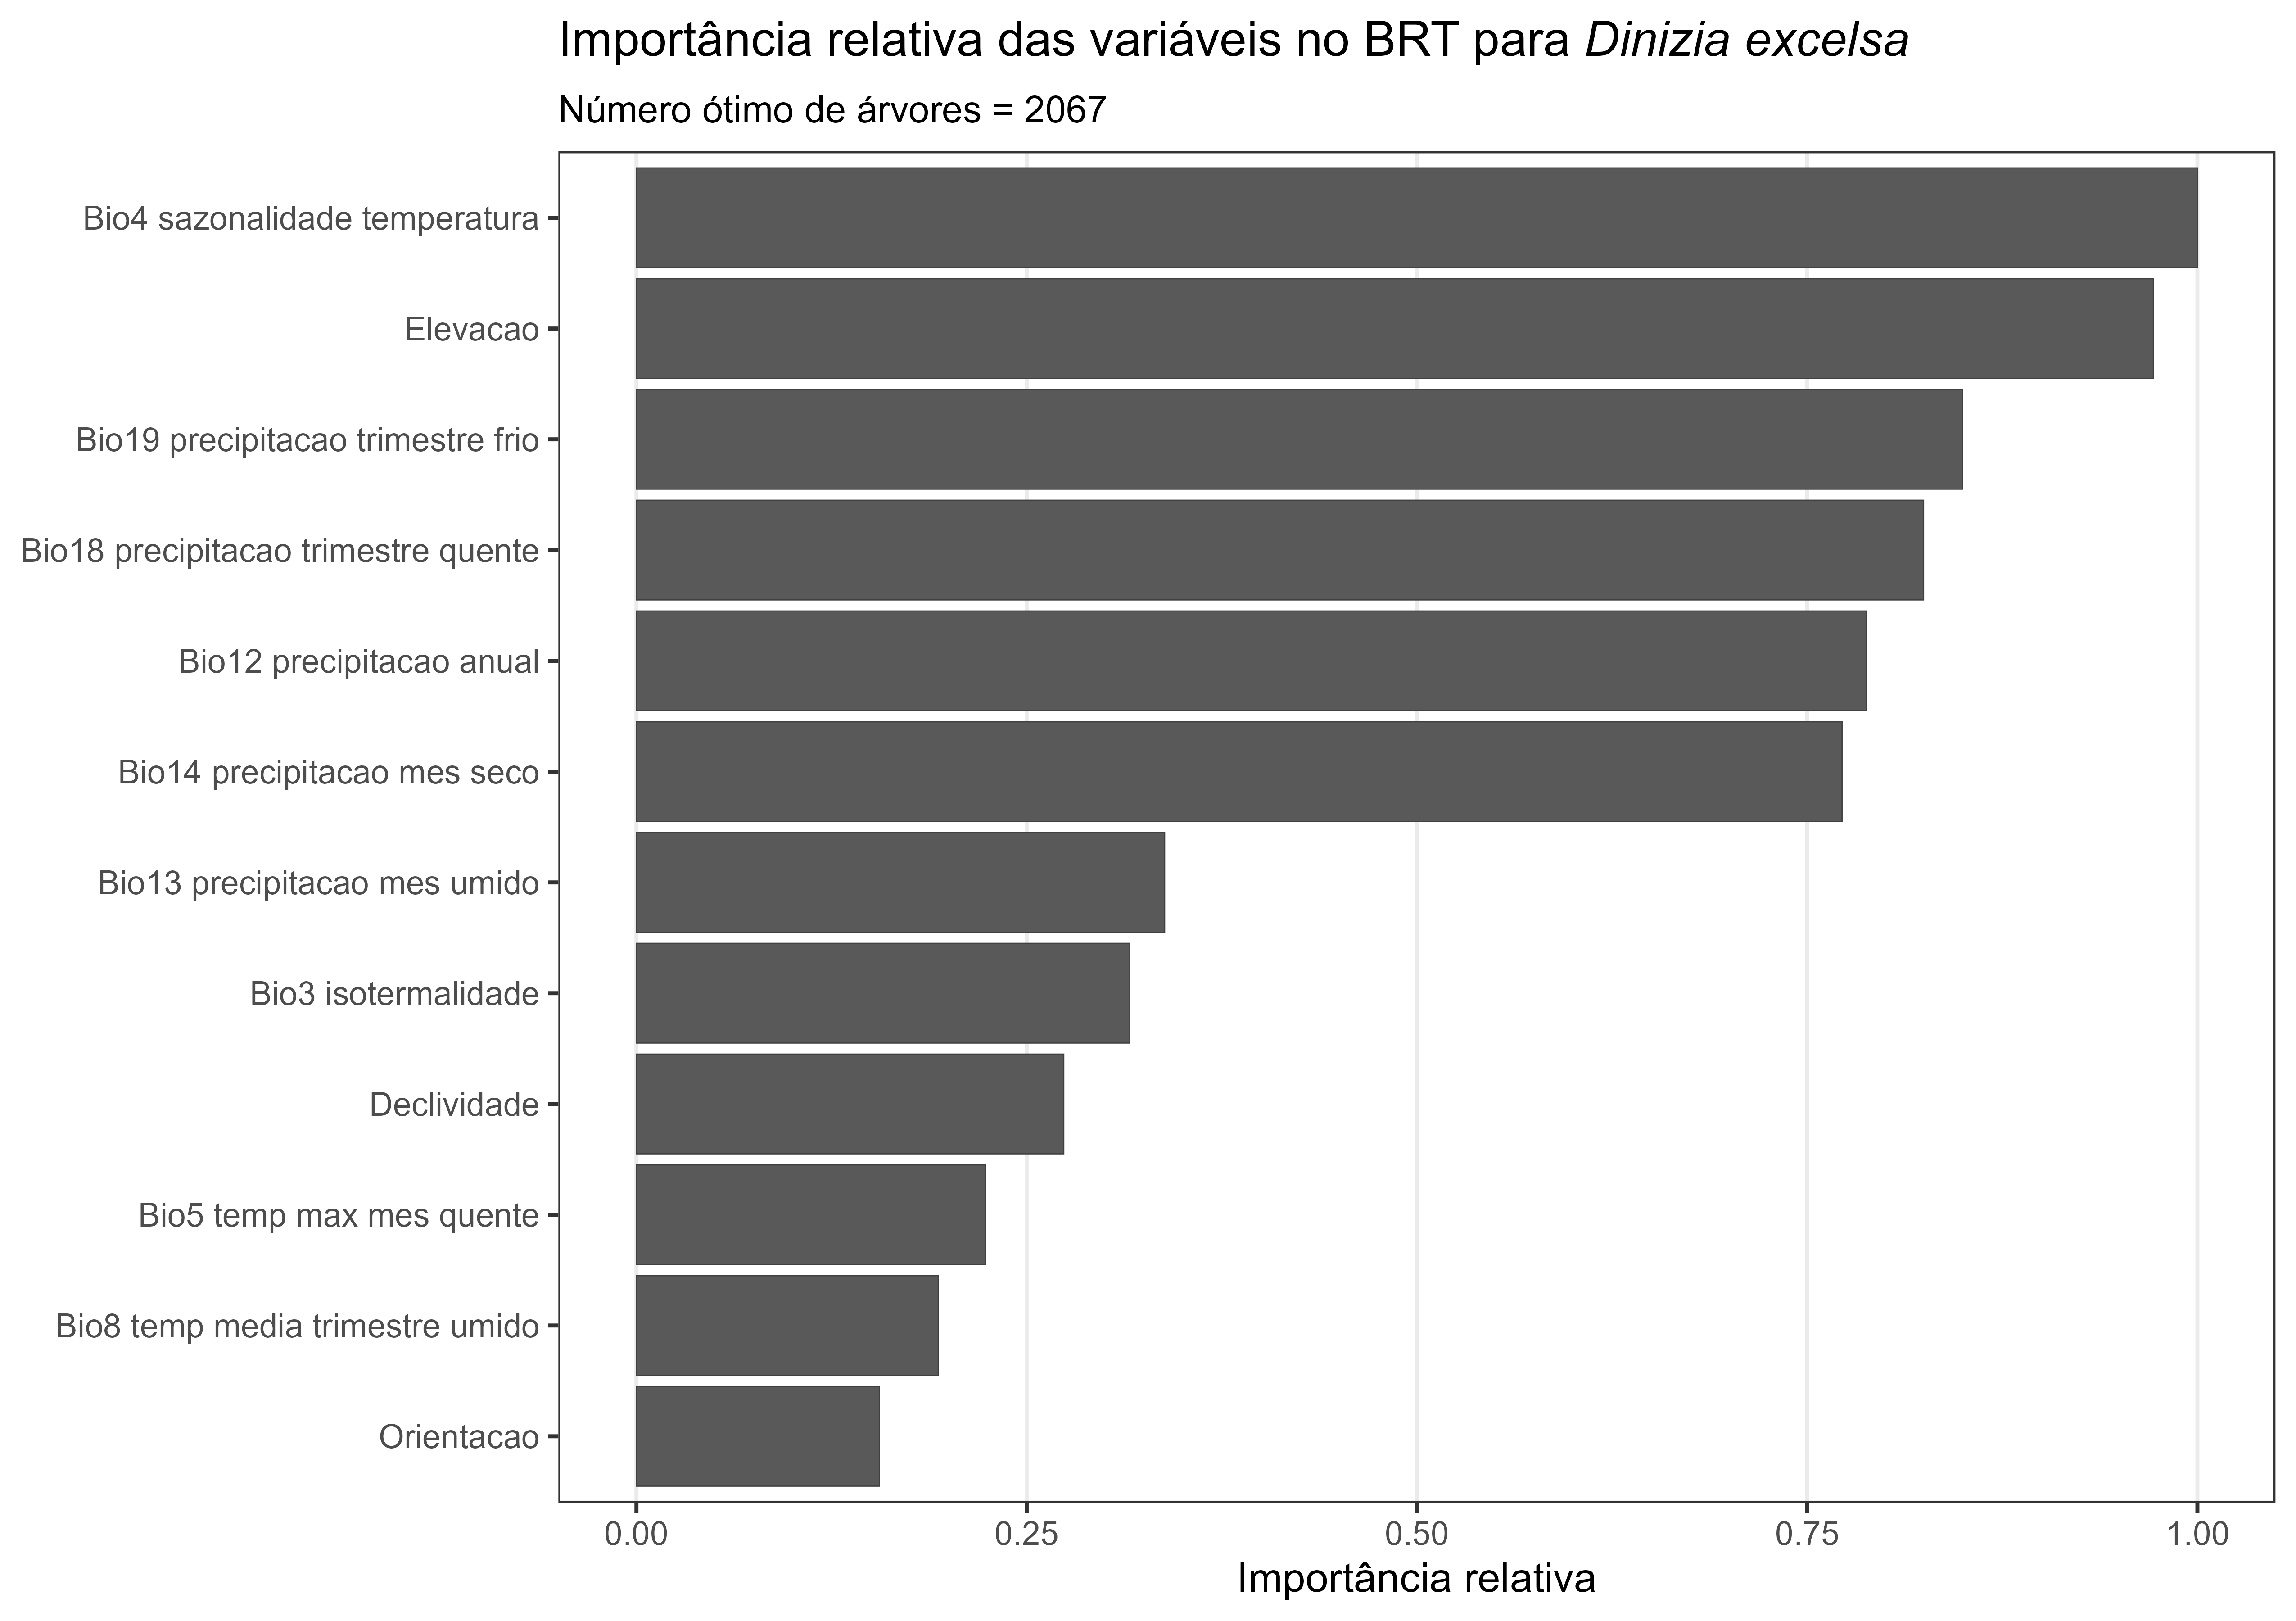
\includegraphics[width=0.86\textwidth]{figuras/unidade09/unidade09_importancia_variaveis_brt.png}
	\caption{Importância relativa das variáveis ambientais no modelo BRT ajustado para \textit{Dinizia excelsa}.}
	\label{fig:unidade09_importancia_brt}
\end{figure}

\section{Avaliação do modelo}

\rscriptfile{scripts/unidade09/04_avaliar_brt_dinizia.R}

\begin{figure}[H]
	\centering
	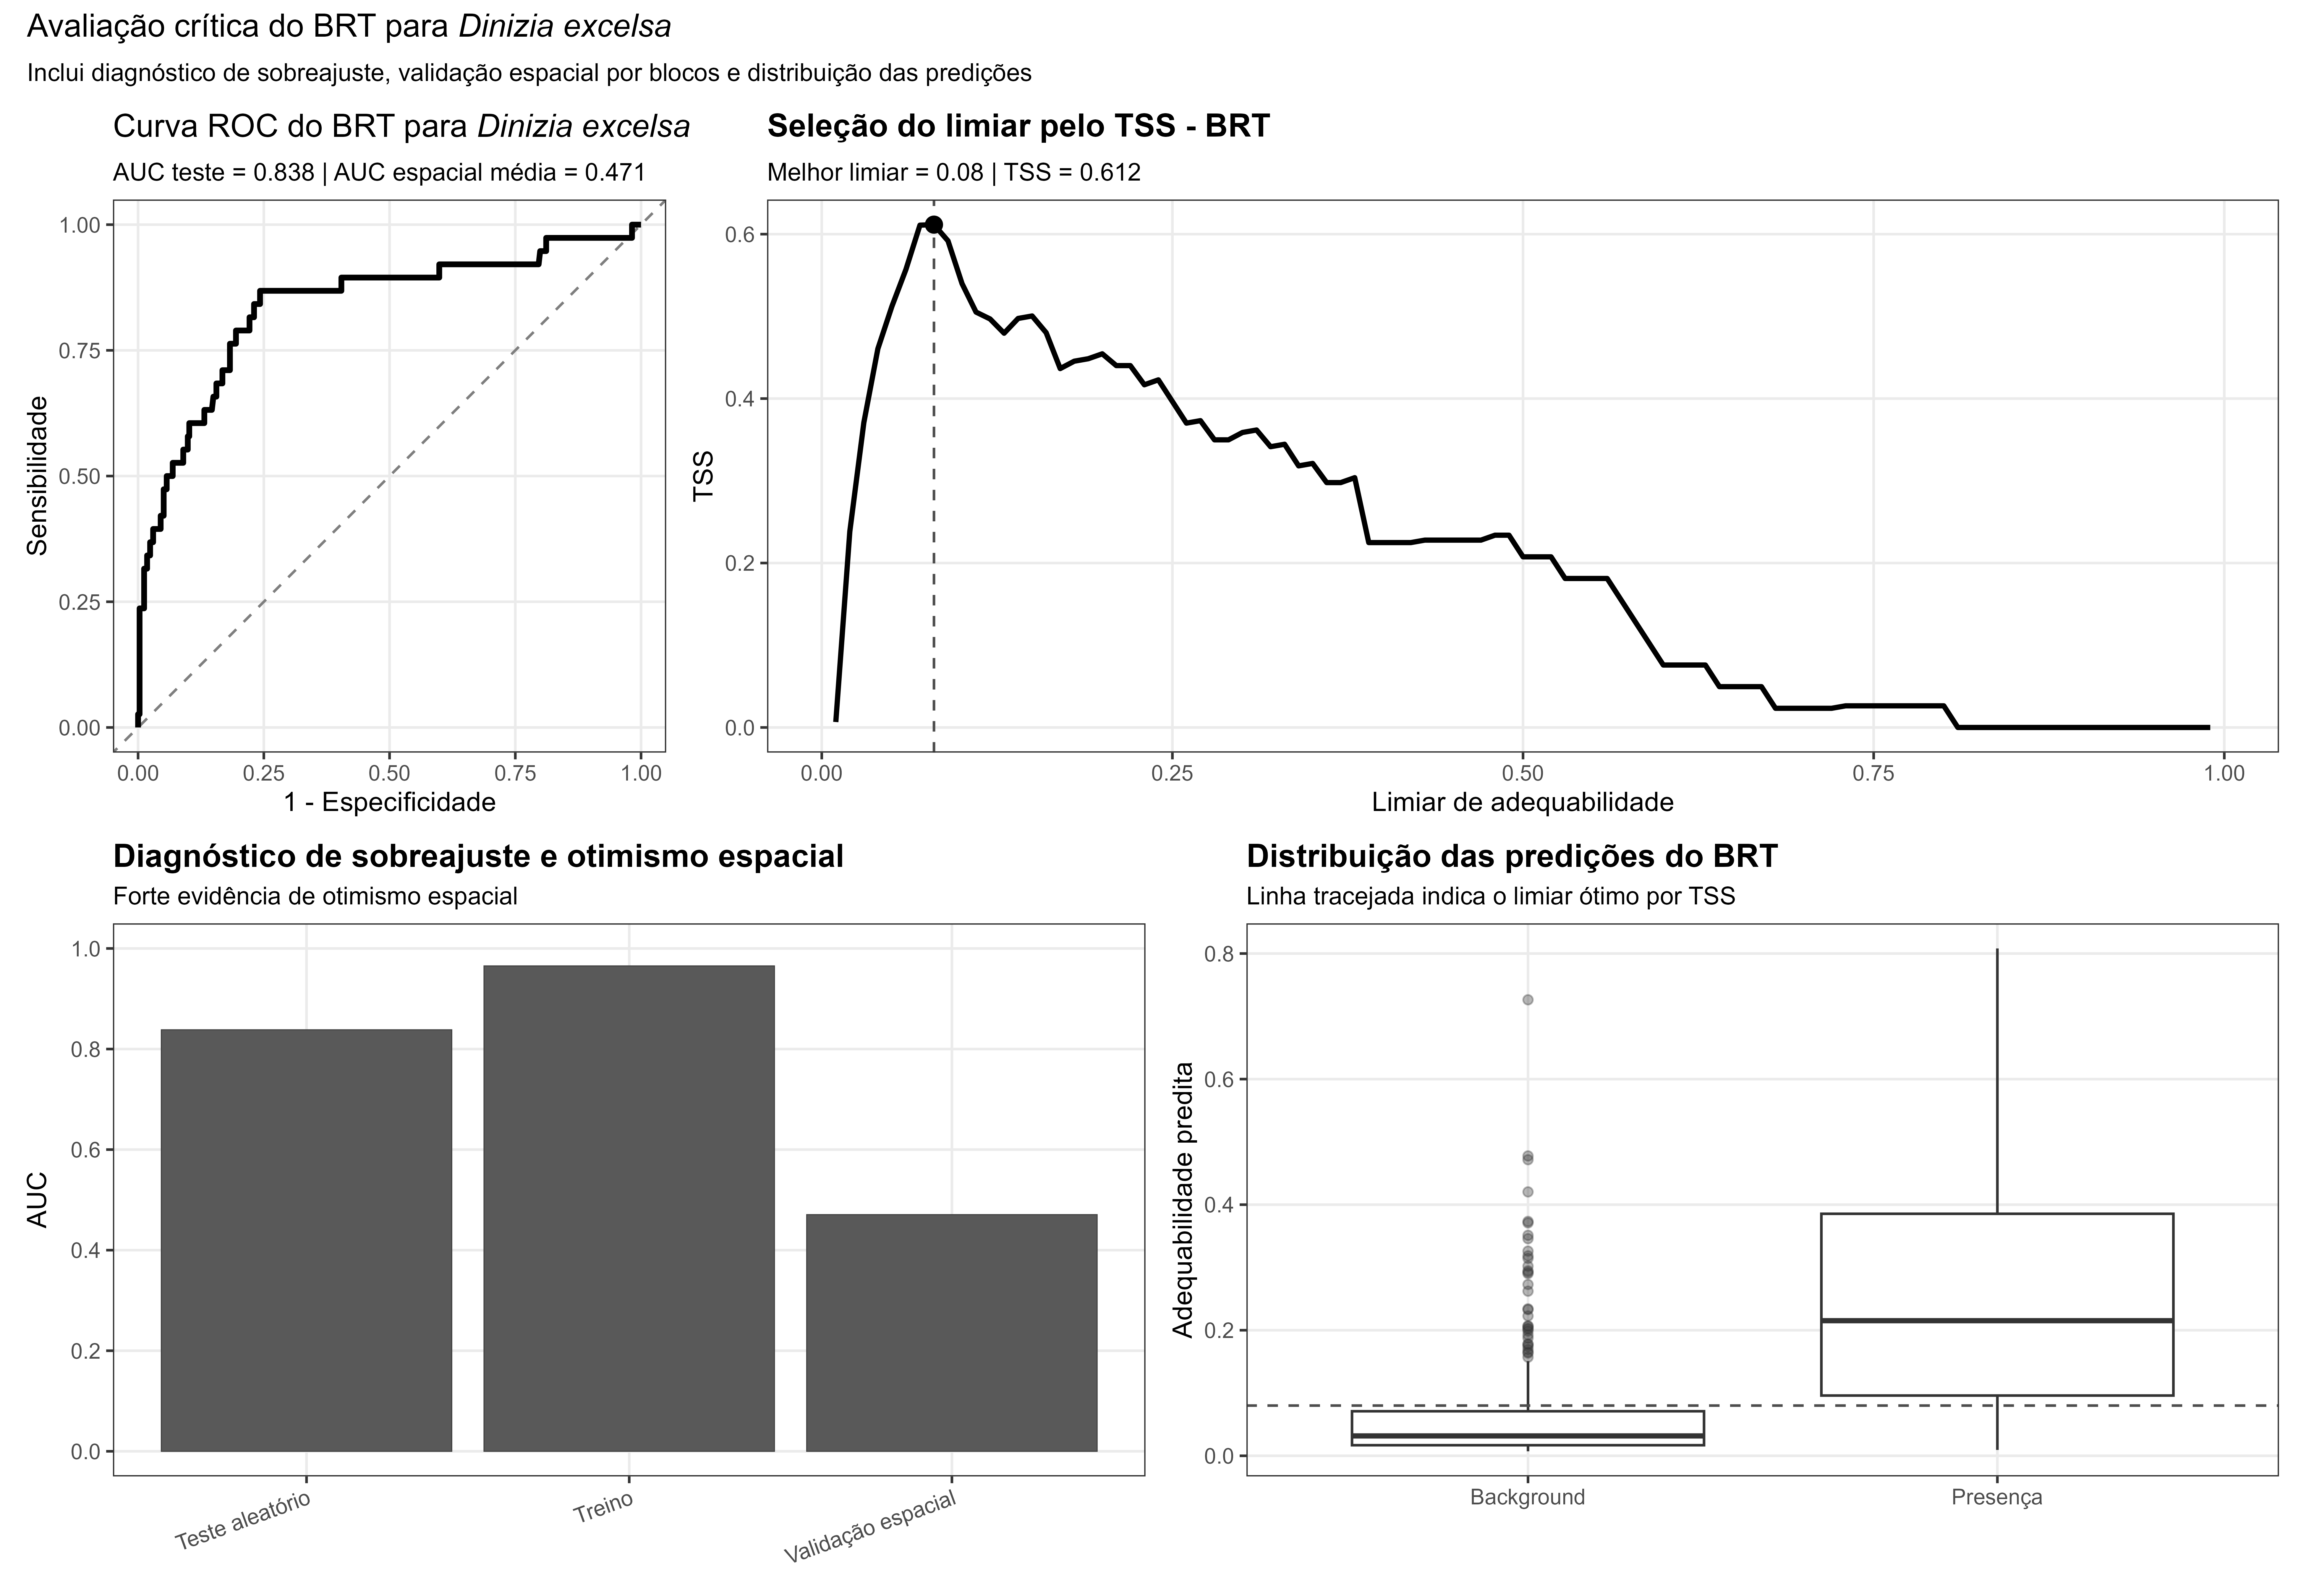
\includegraphics[width=0.78\textwidth]{figuras/unidade09/unidade09_avaliacao_brt_patchwork.png}
	\caption{Curva ROC do BRT avaliado no conjunto teste.}
	\label{fig:unidade09_roc_brt}
\end{figure}

\begin{figure}[H]
	\centering
	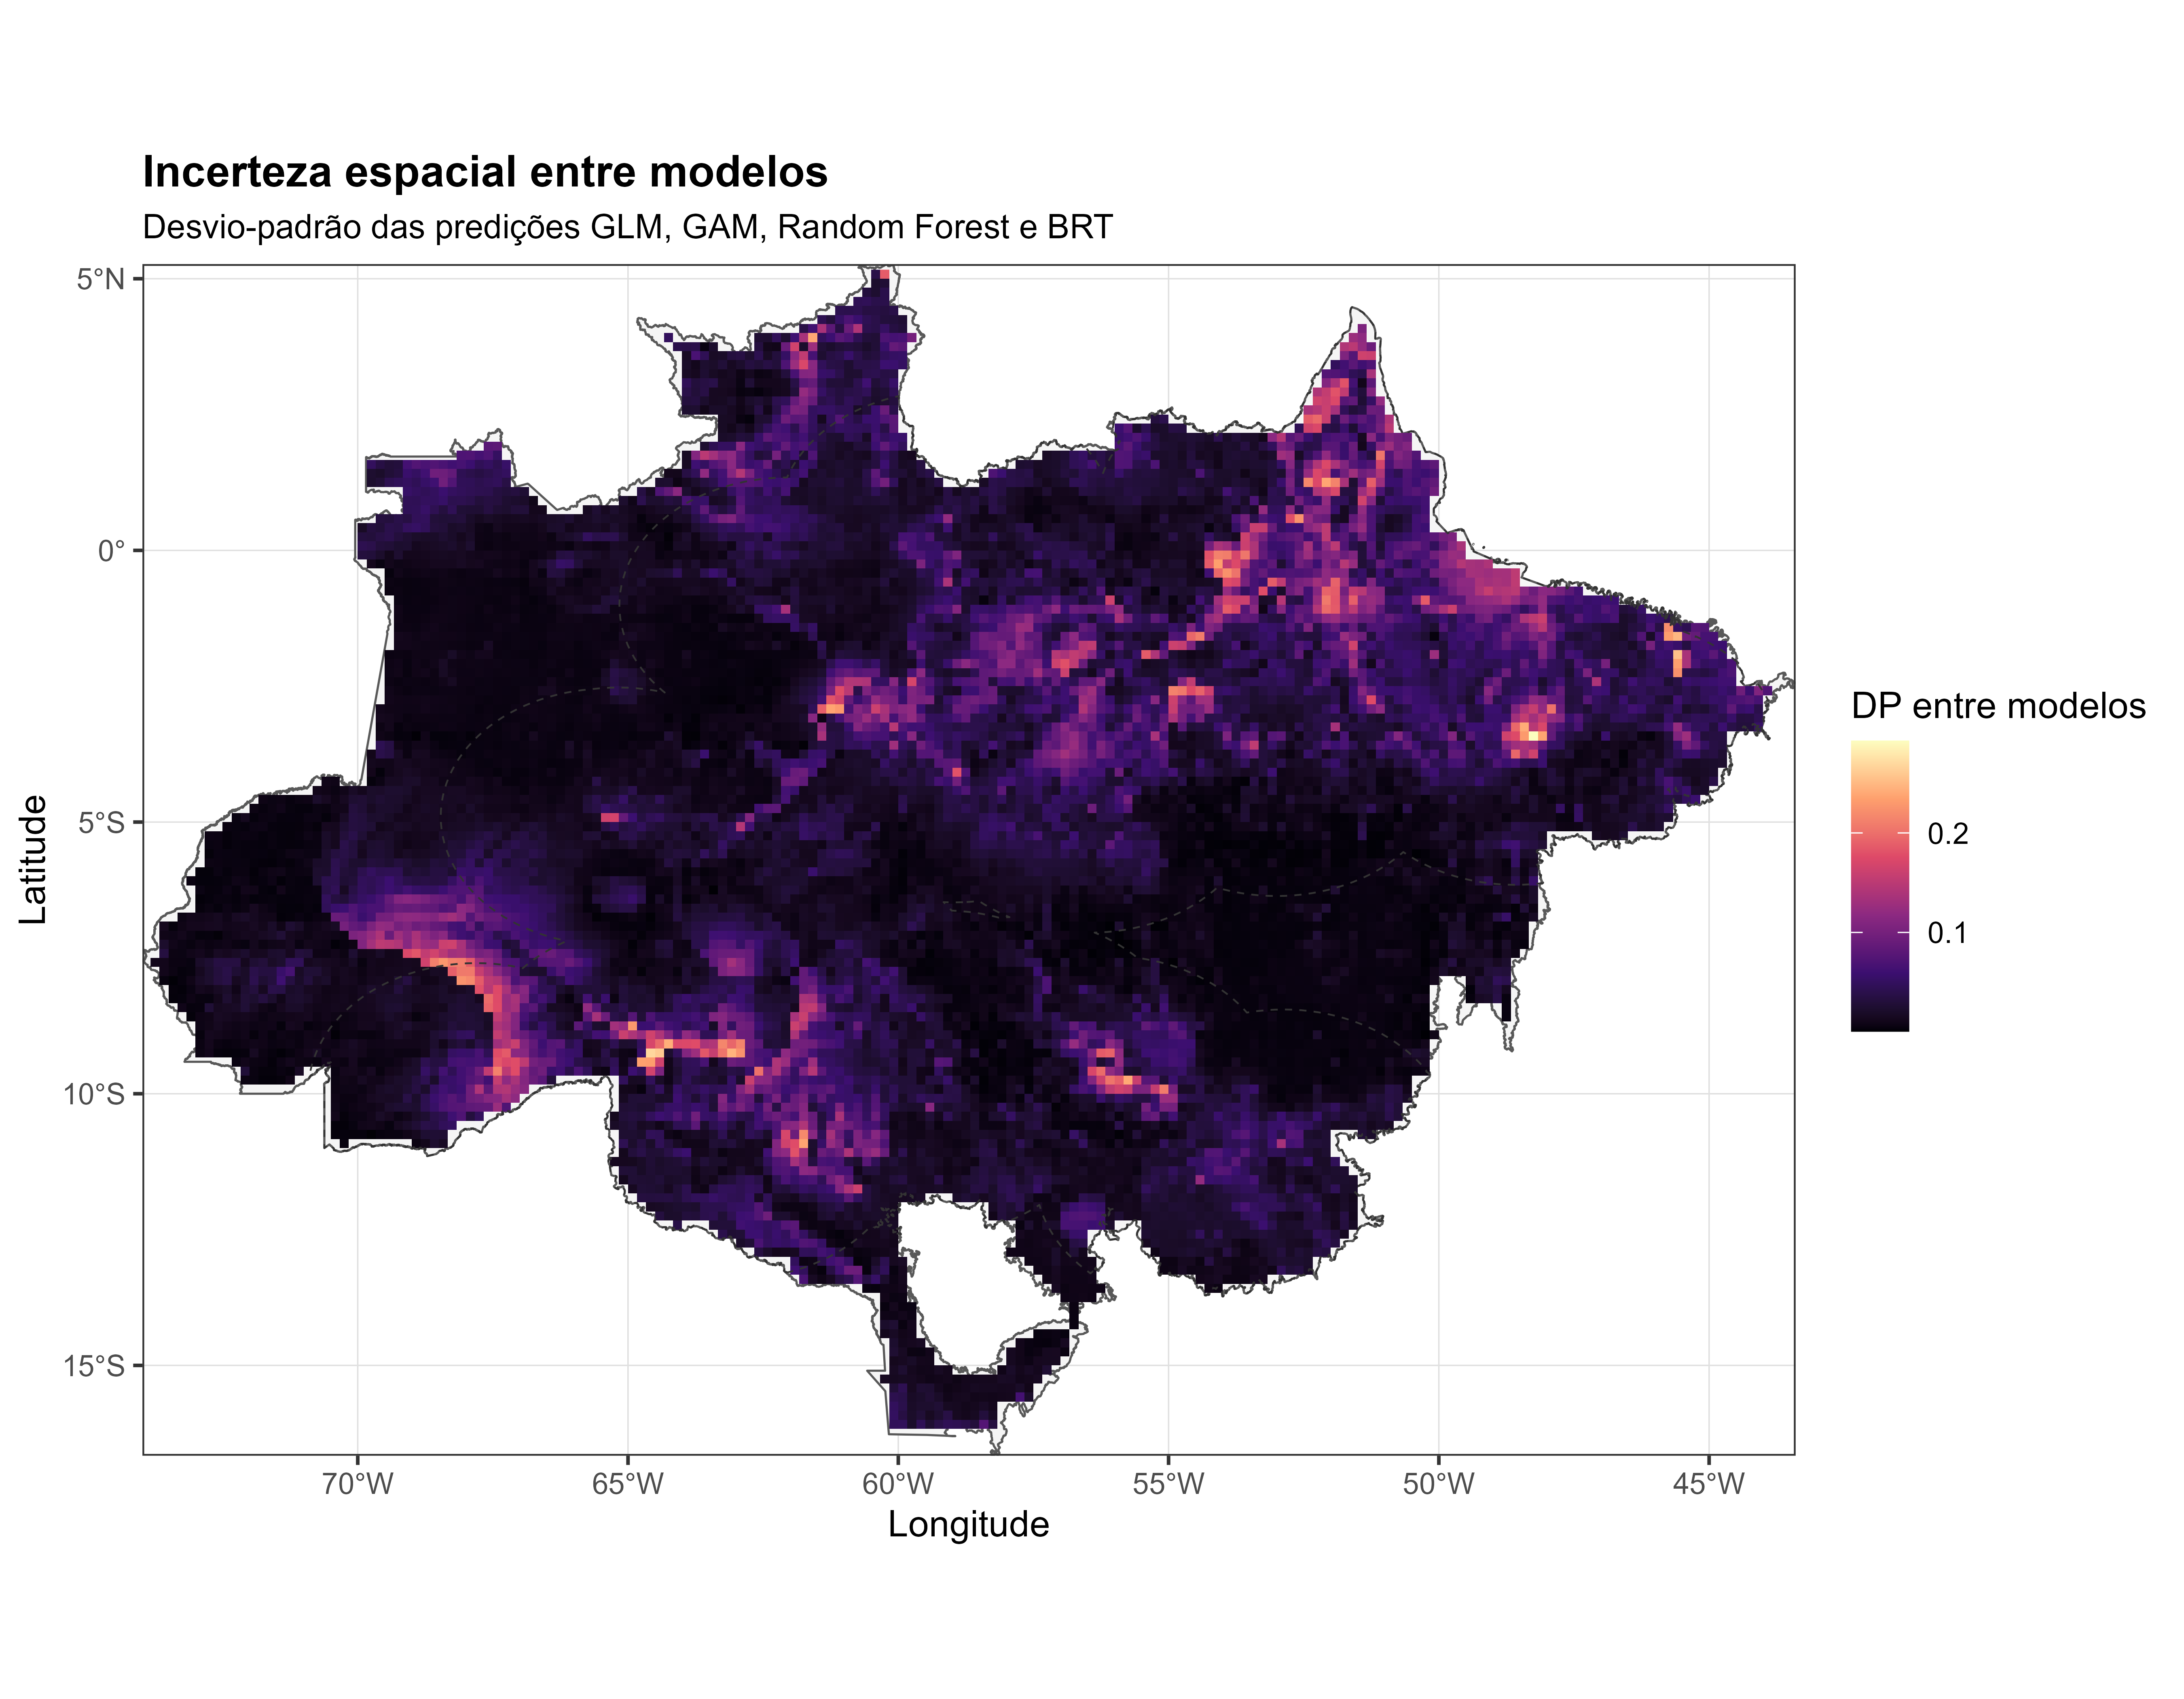
\includegraphics[width=0.78\textwidth]{figuras/unidade09/unidade09_incerteza_sd_glm_gam_rf_brt.png}
	\caption{Incerteza associada às predições de distribuição potencial de \textit{Dinizia excelsa}, calculada como o desvio-padrão entre os modelos GLM, GAM, Random Forest e BRT. Áreas com maiores valores indicam menor consenso entre algoritmos e, consequentemente, maior incerteza preditiva, enquanto áreas com baixos valores representam regiões de elevada concordância entre modelos.}
	\label{fig:unidade09_incerteza_brt}
\end{figure}

\section{Mapa de adequabilidade atual}

\rscriptfile{scripts/unidade09/05_predicao_espacial_brt.R}

\begin{figure}[H]
	\centering
	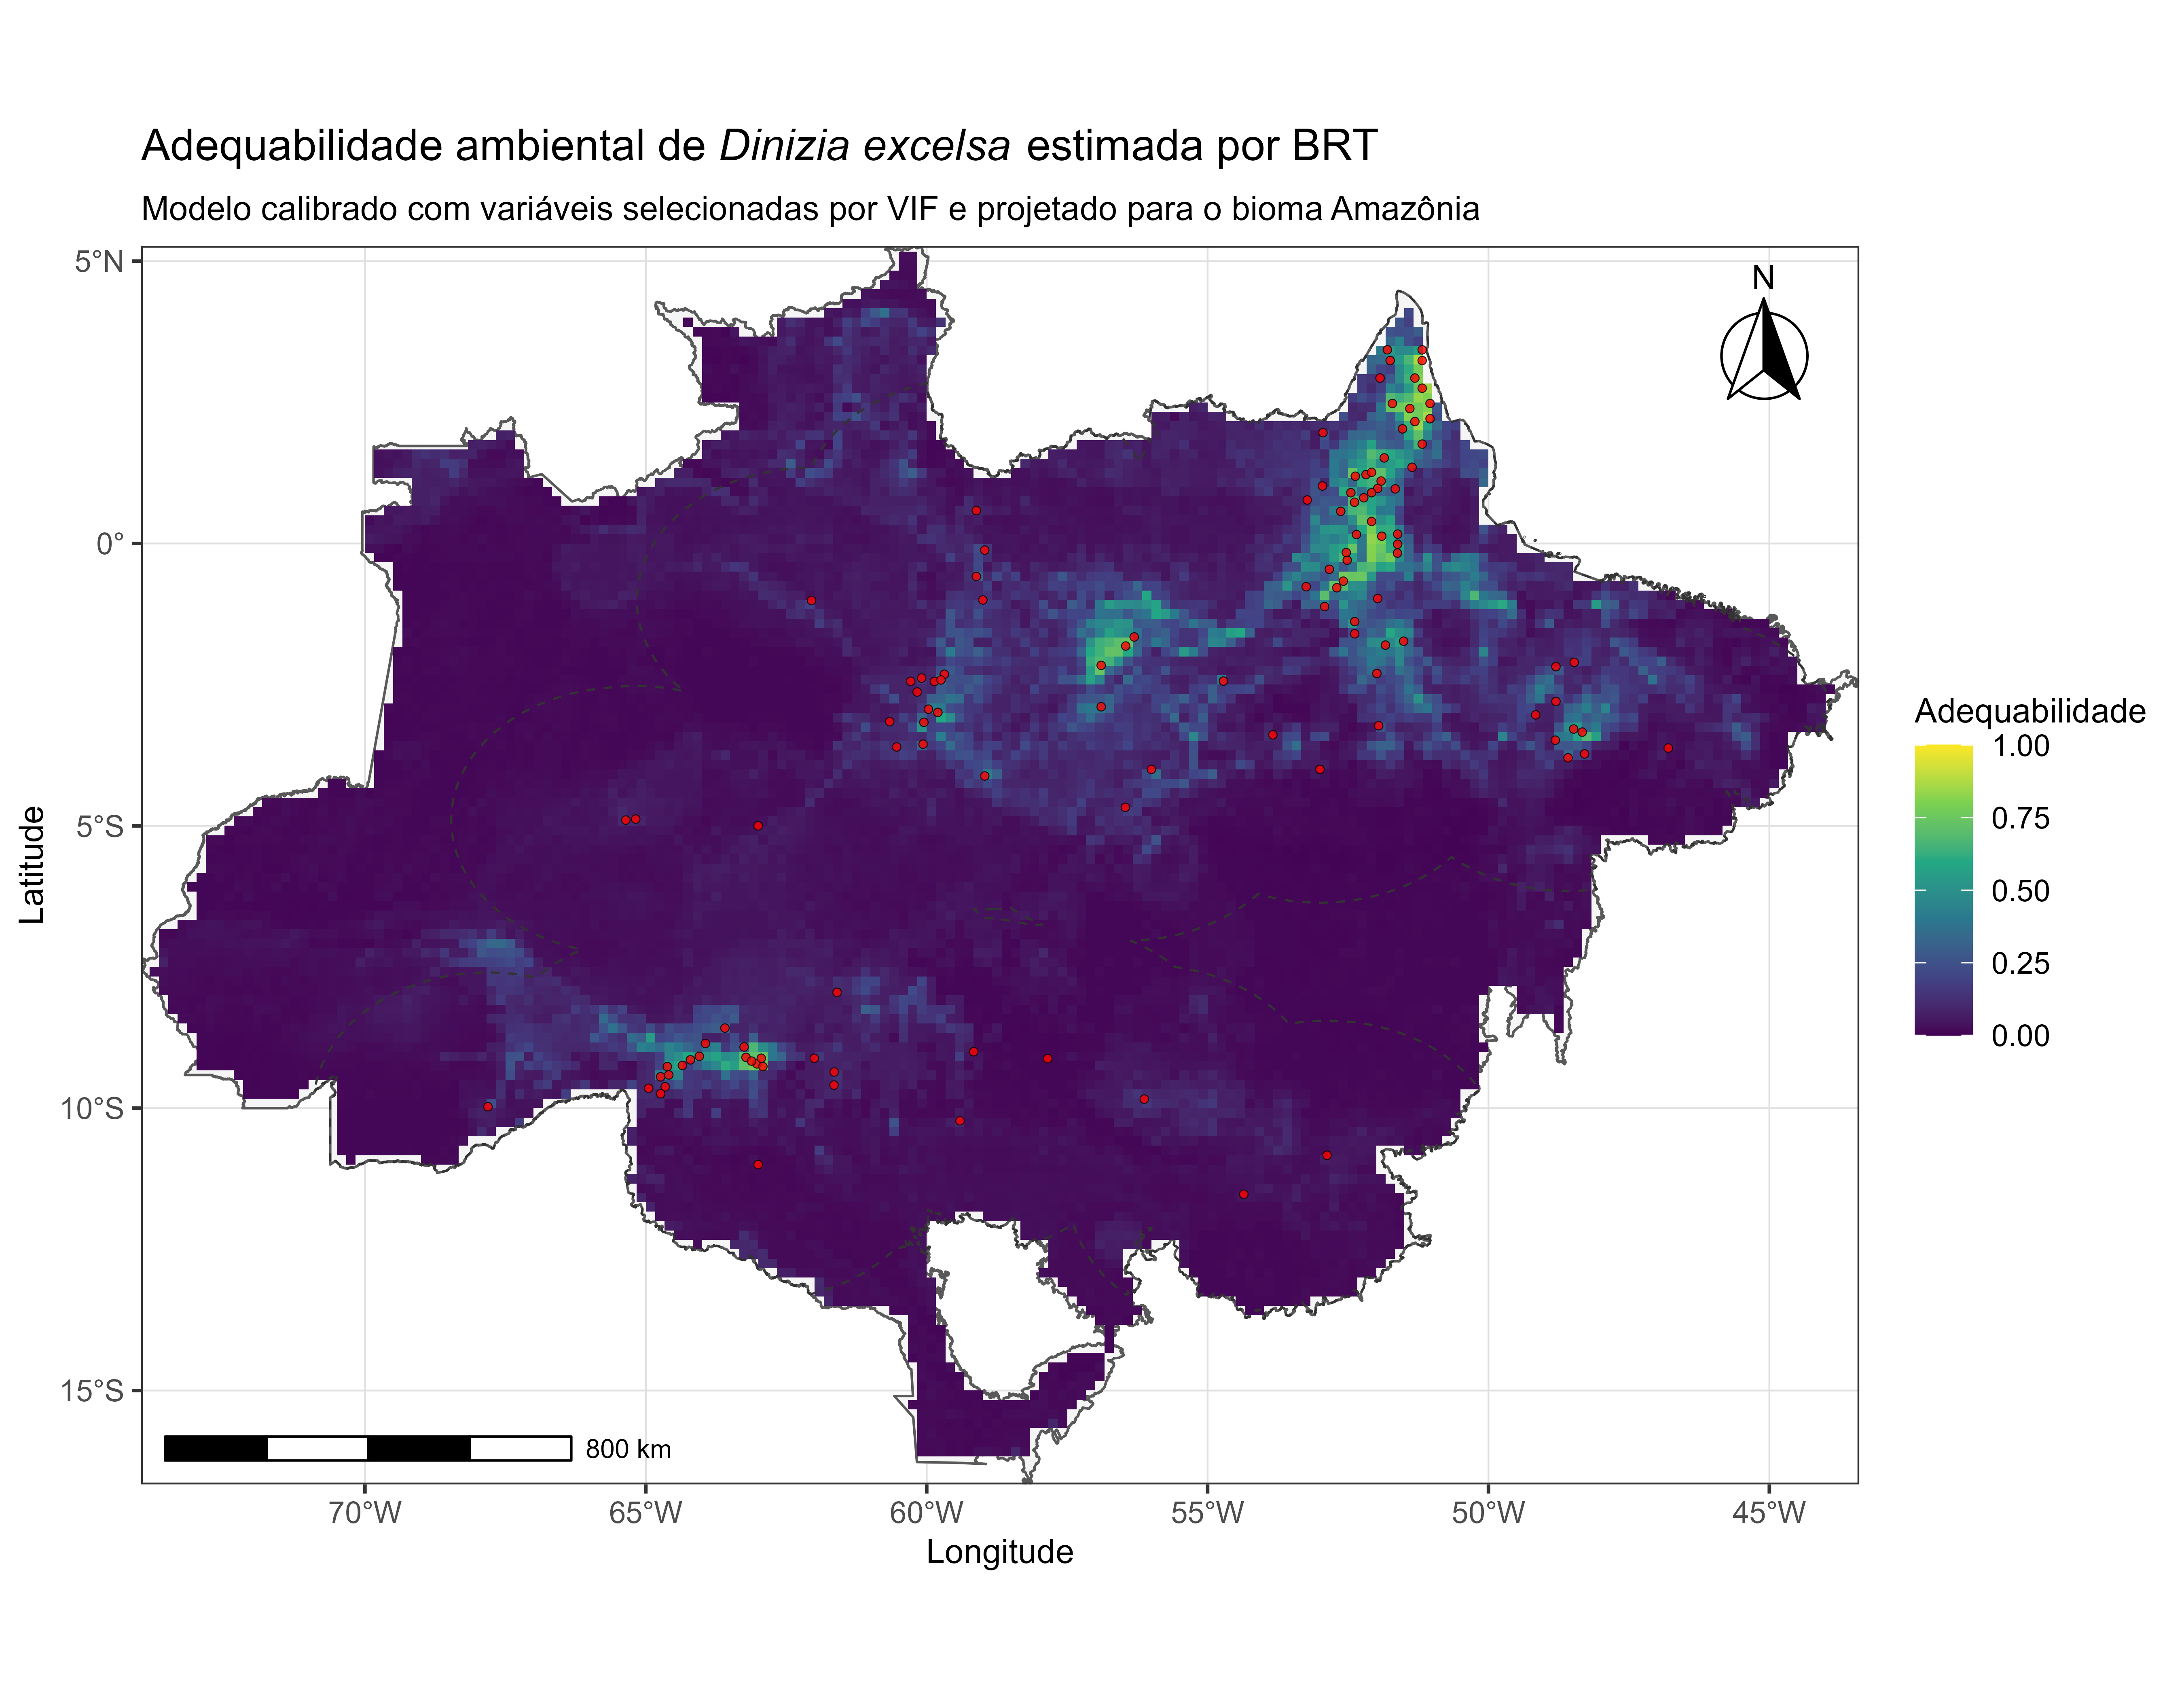
\includegraphics[width=0.88\textwidth]{figuras/unidade09/unidade09_adequabilidade_brt.png}
	\caption{Mapa de adequabilidade ambiental atual de \textit{Dinizia excelsa} estimado por BRT dentro da área acessível \(M\).}
	\label{fig:unidade09_adequabilidade_brt}
\end{figure}

\section{Curvas de resposta parcial}

\rscriptfile{scripts/unidade09/06_curvas_resposta_brt.R}

\begin{figure}[H]
	\centering
	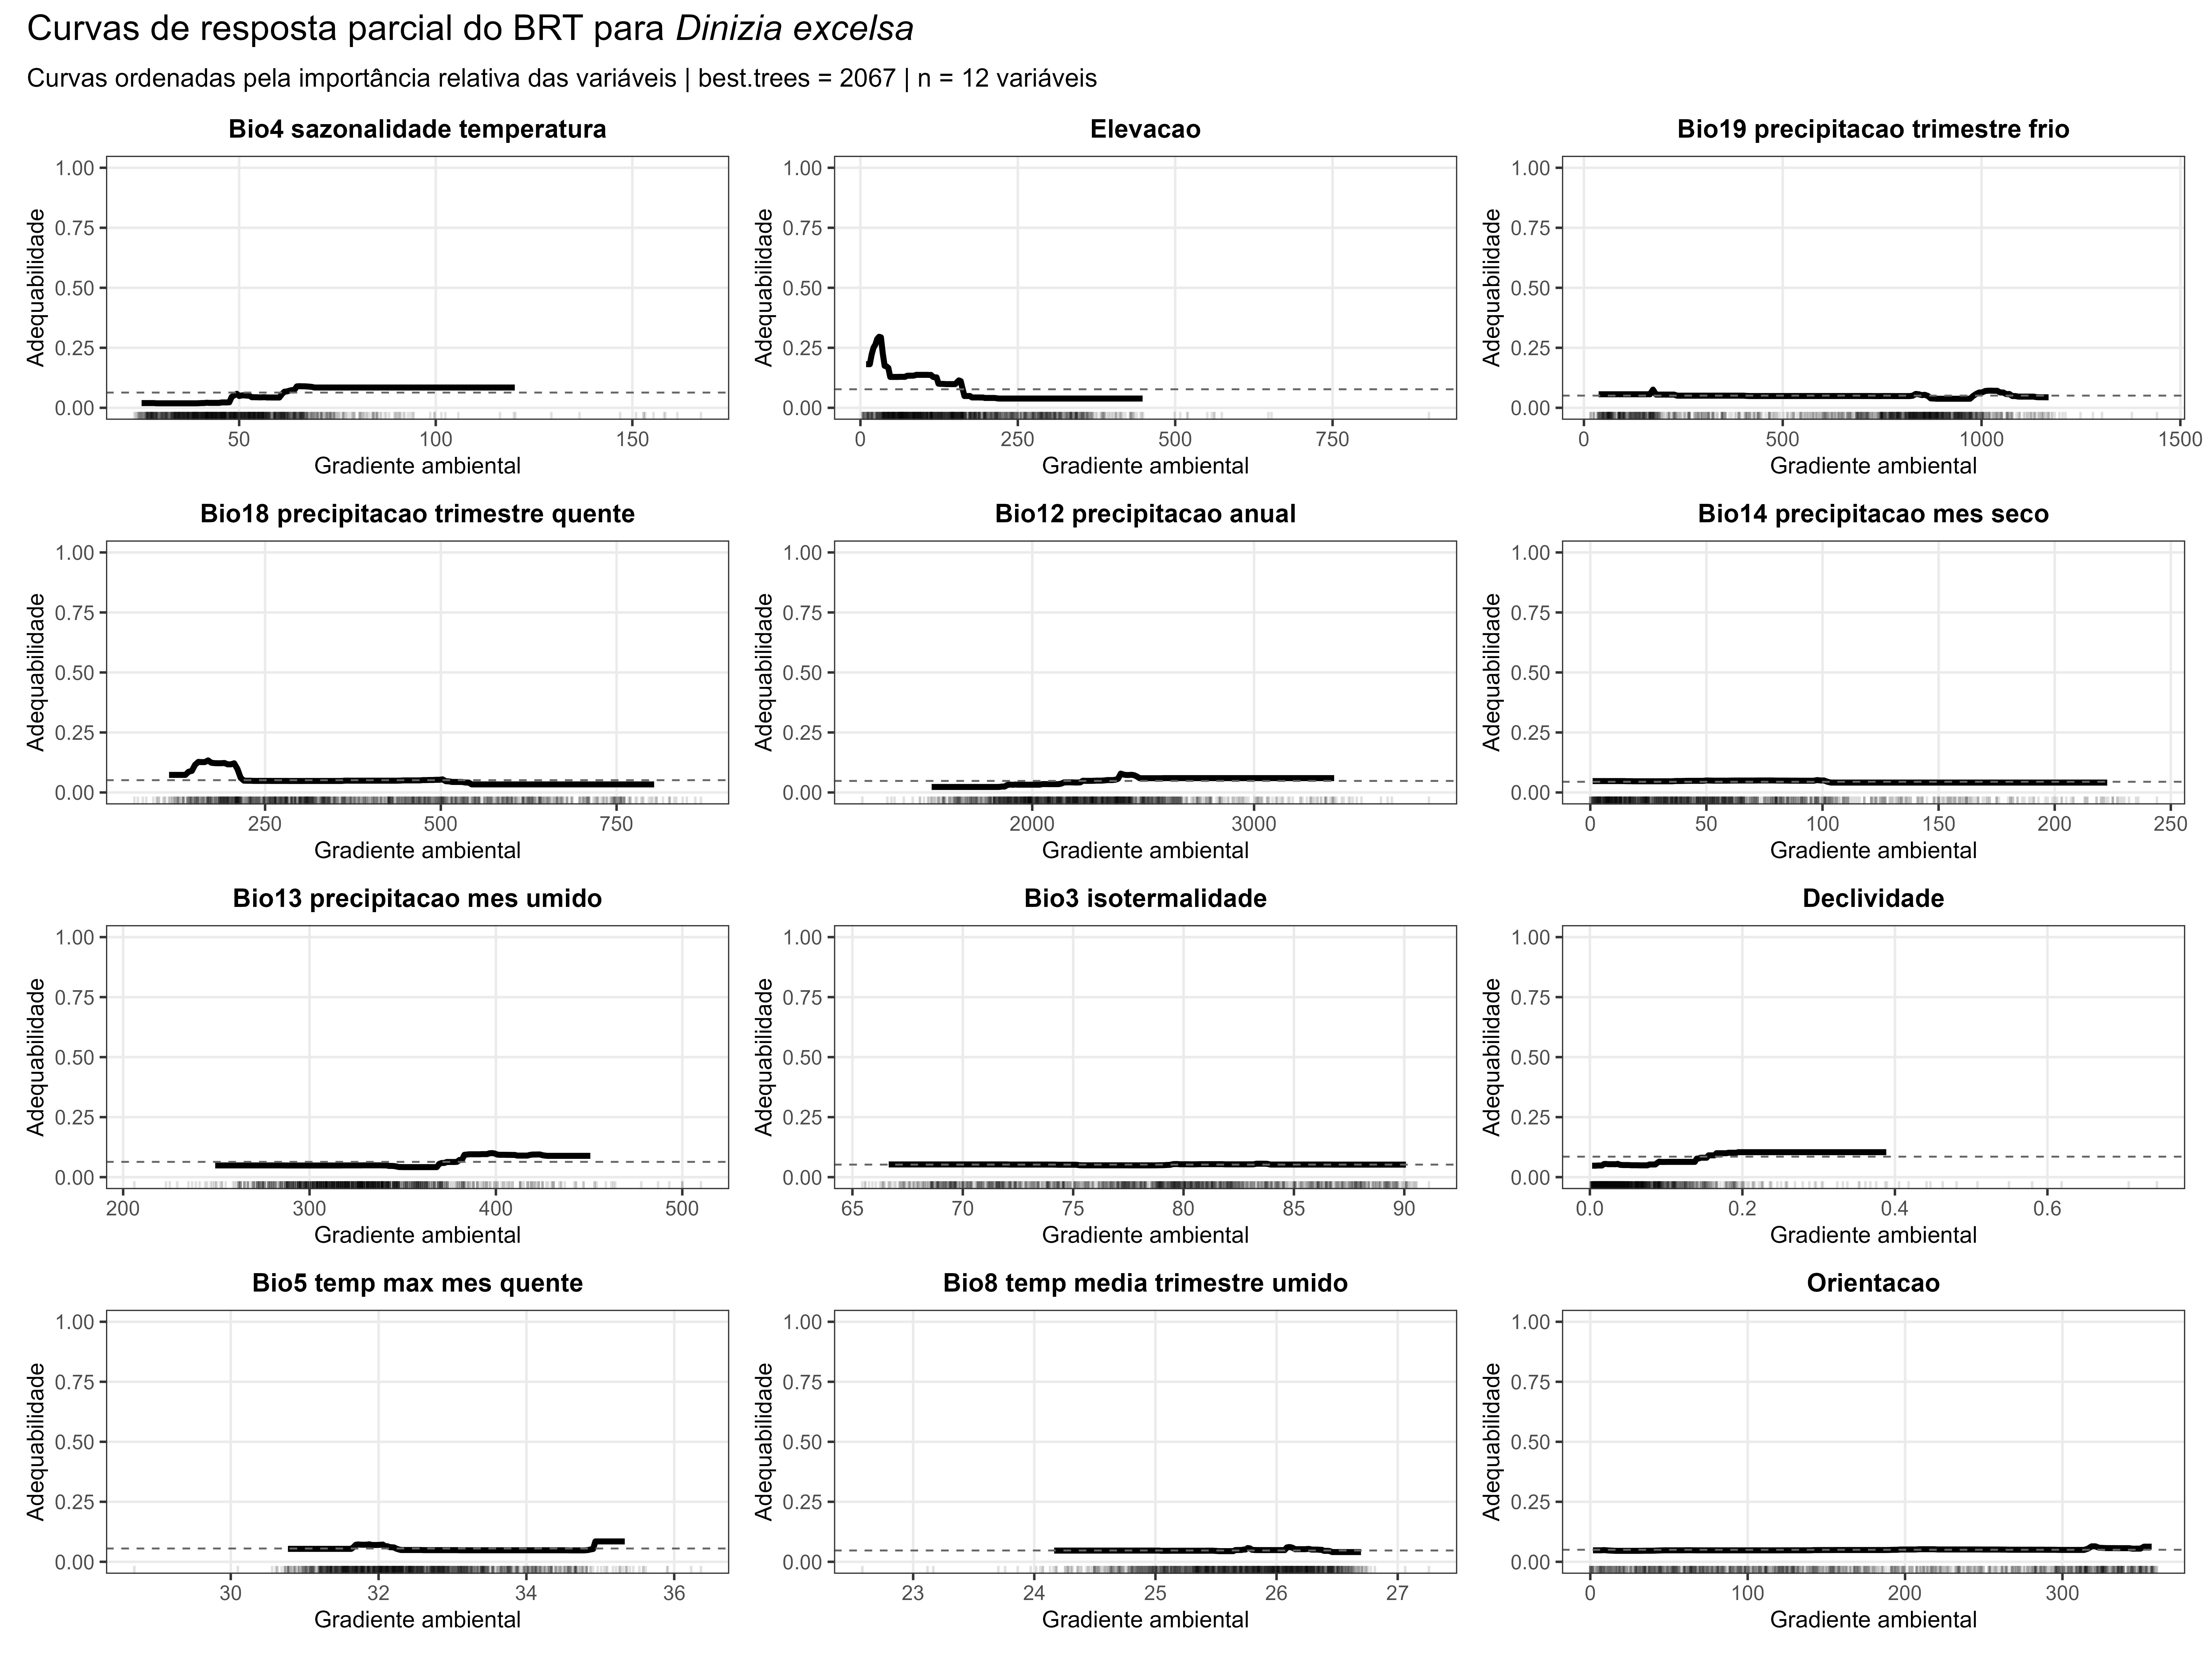
\includegraphics[width=0.96\textwidth]{figuras/unidade09/unidade09_curvas_resposta_brt.png}
	\caption{Curvas de resposta parcial do BRT para as variáveis ambientais selecionadas.}
	\label{fig:unidade09_curvas_resposta_brt}
\end{figure}

\section{Comparação com GLM, GAM e Random Forest}

\rscriptfile{scripts/unidade09/07_comparar_modelos_brt.R}

\begin{figure}[H]
	\centering
	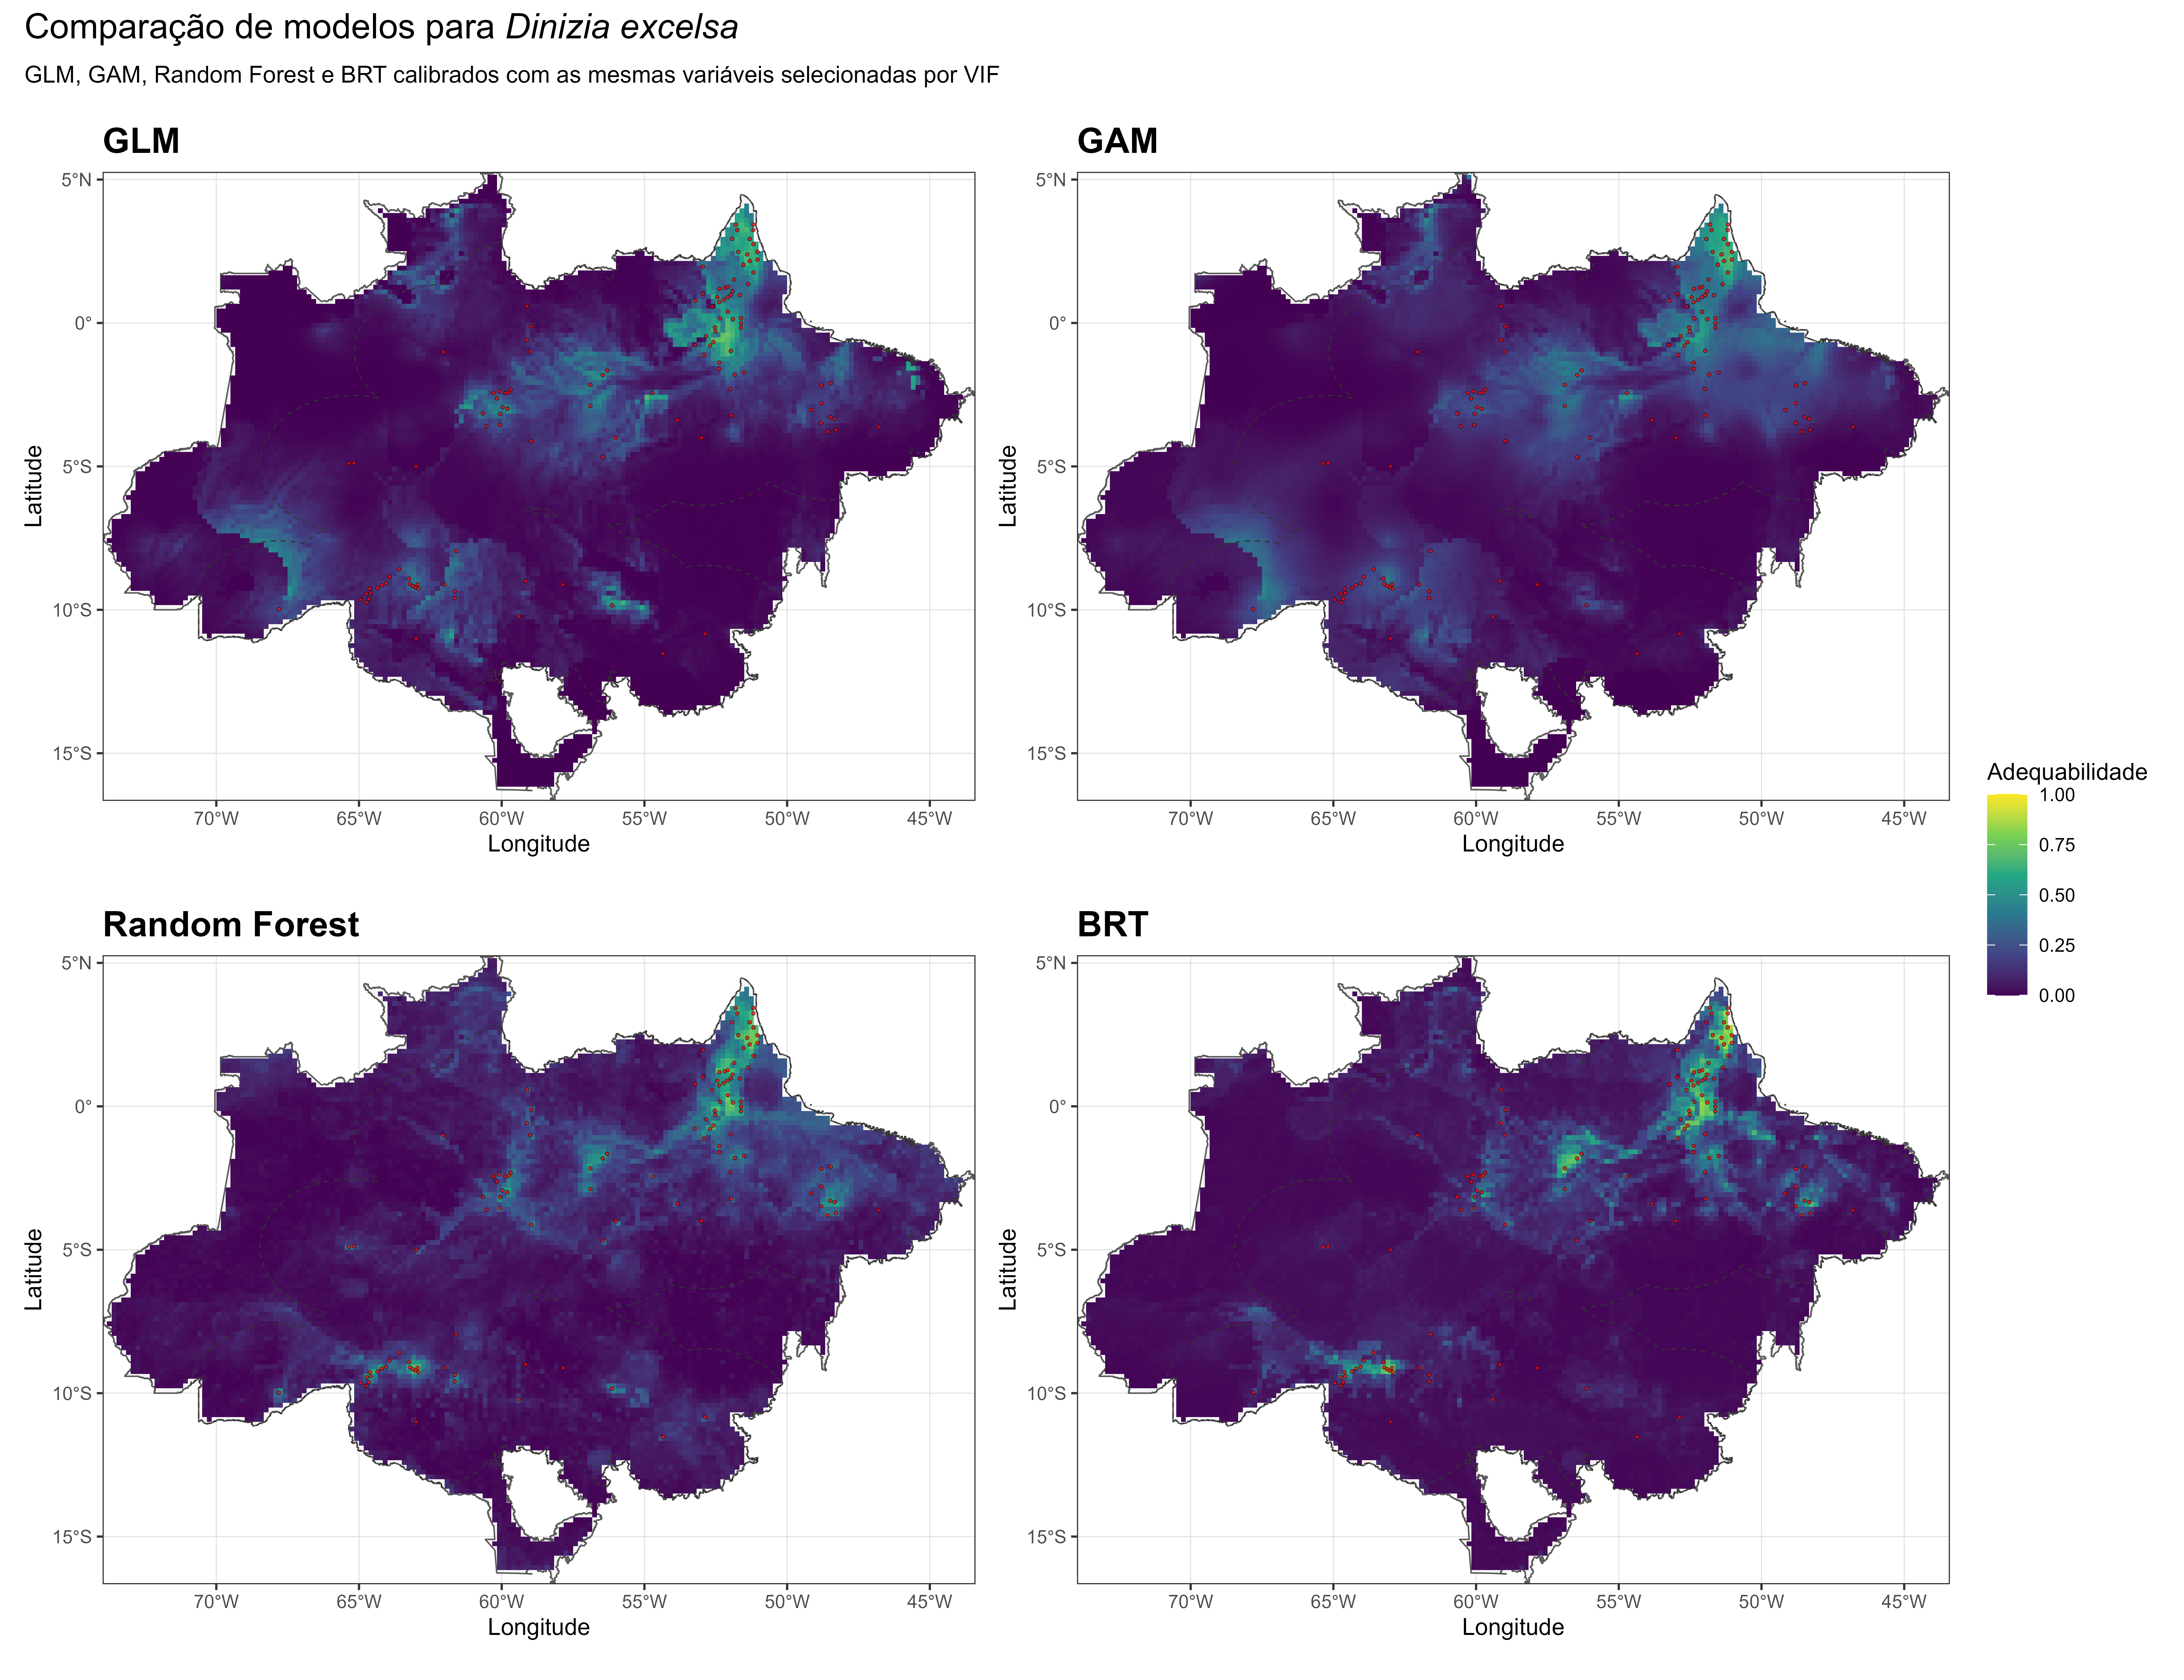
\includegraphics[width=0.96\textwidth]{figuras/unidade09/unidade09_comparacao_glm_gam_rf_brt.png}
	\caption{Comparação entre mapas de adequabilidade estimados por GLM, GAM, Random Forest e BRT.}
	\label{fig:unidade09_comparacao_modelos}
\end{figure}

\section{Pipeline completo}

\rscriptfile{scripts/unidade09/08_pipeline_brt.R}

\section{Síntese da unidade}

BRT é um algoritmo poderoso para SDM por combinar flexibilidade, capacidade de modelar interações e boa performance preditiva. Entretanto, seu uso exige cautela metodológica, especialmente no controle de hiperparâmetros e na avaliação em dados independentes.

\begin{conceito}[title={\faBook\quad Mensagem central}]
	BRT pode revelar respostas ambientais complexas, mas sua credibilidade depende de validação adequada, controle de sobreajuste e interpretação ecológica das respostas estimadas.
\end{conceito}

\section{Exercícios de fixação}

\begin{enumerate}
	\item Explique a diferença entre Random Forest e BRT.
	\item O que significa boosting?
	\item Por que o parâmetro \texttt{shrinkage} é importante?
	\item Qual o papel de \texttt{interaction.depth}?
	\item Por que o número ótimo de árvores deve ser selecionado por validação cruzada?
	\item Como interpretar a importância relativa das variáveis em BRT?
	\item Por que curvas de resposta parcial devem ser avaliadas criticamente?
\end{enumerate}

% ============================================================
% UNIDADE 10
% ============================================================

